\chapter{Scale-Covariant Collisionless Boltzmann Dynamics and Late-Time Observables}
\PhysicsContext{From a distribution to observables}{The third part carries one prescribed distribution through momentum-resolved transport, photon and neutrino hierarchies, recombination, reionization, line-of-sight projection, and CMB lensing. These are controlled templates, not a precision replacement for production codes.}


\label{ch:collisionless-boltzmann-observables}

\section{Scope and objective}

The scale-covariant refinement dark sector fixes a discrete mass spectrum, a production distribution, a cold late-time limit, and a density-dependent locking source.  The preceding growth calculation replaced that distribution by one adiabatic sound speed.  That fluid closure is adequate on large scales but does not retain momentum dependence, free streaming, or the higher angular moments of the collisionless distribution.

This chapter develops the kinetic layer in two stages.  First, it derives the complete linear collisionless hierarchy for every retained refinement level and momentum node.  Second, it specializes that hierarchy to a controlled post-recombination, subhorizon Einstein--Vlasov--Poisson system and propagates one fixed scale-covariant distribution into matter-power, redshift-space-growth, weak-lensing, and CMB-lensing templates.

The numerical section begins at
\begin{equation}
 a_i=10^{-3}.
 \label{eq:cb-initial-scale}
\end{equation}
Adiabatic perturbations are prescribed at that surface.  The calculation therefore measures the \emph{incremental post-recombination transfer} generated between $a_i$ and today; it does not evolve free streaming from the production event to $a_i$.  Radiation is retained in the background expansion but its perturbations are not included in the late-time Poisson source.  Consequently the section does not compute primary CMB temperature or polarization spectra, recombination kinetics, neutrino transport, or superhorizon metric evolution.  The CMB result below is a late-time lensing template and a scale-separation diagnostic, not a primary-anisotropy likelihood.

\section{Scale-covariant phase-space distribution}

For each retained detail level $h$, let
\begin{equation}
 m_h=\Lambda p^{\sigma h},
 \qquad
 d_h=(p-1)p^{h-1},
 \label{eq:cb-level-data}
\end{equation}
within the high-level scale-covariant branch.  The rapid-crossing distribution has the form
\begin{equation}
 \bar f_h(q)
 =\eta\exp\left[-\frac{\pi m_h^2}{\nu_h}
 -\frac{\pi q^2}{a_\star^2\nu_h}\right],
 \qquad
 \nu_h=A_\star m_h.
 \label{eq:cb-background-distribution}
\end{equation}
For the benchmark used here, $A_\star$ is the mass unit, $p=2$, $\sigma=1$, and
\begin{equation}
 \frac{\Lambda}{A_\star}=10^{-4},
 \qquad
 a_\star=10^{-6}.
 \label{eq:cb-benchmark-production}
\end{equation}
The common energy-projection normalization $\eta$ cancels from every linear transfer ratio.

The conformal energy is
\begin{equation}
 \epsilon_h(q,a)=\sqrt{q^2+a^2m_h^2},
 \label{eq:cb-conformal-energy}
\end{equation}
and the background density and pressure are
\begin{equation}
 \rho_h(a)
 =\frac{d_h}{2\pi^2a^4}
 \int_0^\infty q^2\epsilon_h\bar f_h\,dq,
 \label{eq:cb-background-density}
\end{equation}
\begin{equation}
 p_h(a)
 =\frac{d_h}{6\pi^2a^4}
 \int_0^\infty \frac{q^4}{\epsilon_h}\bar f_h\,dq.
 \label{eq:cb-background-pressure}
\end{equation}
The numerical phase grid retains the ten levels carrying all but less than $10^{-6}$ of the present rest-density weight.  Their retained weights sum to unity to $2.3\times10^{-16}$.

\section{Complete linear collisionless hierarchy}

Use conformal Newtonian gauge,
\begin{equation}
 ds^2=a^2(\eta)
 \left[-(1+2\Psi)d\eta^2+(1-2\Phi)d\mathbf x^2\right].
 \label{eq:cb-newtonian-gauge}
\end{equation}
Write the perturbed distribution as
\begin{equation}
 f_h(\mathbf k,q,\mu,\eta)
 =\bar f_h(q)
 \left[1+\mathcal F_h(\mathbf k,q,\mu,\eta)\right],
 \label{eq:cb-distribution-perturbation}
\end{equation}
where $\mu=\widehat{\mathbf k}\cdot\widehat{\mathbf q}$, and expand
\begin{equation}
 \mathcal F_h
 =\sum_{\ell\geq0}
 (-i)^\ell(2\ell+1)
 F_{h\ell}(k,q,\eta)P_\ell(\mu).
 \label{eq:cb-multipole-expansion}
\end{equation}
Set
\begin{equation}
 D_h(q):=\frac{d\log\bar f_h}{d\log q}.
 \label{eq:cb-log-derivative}
\end{equation}
The linear collisionless Boltzmann equation gives
\begin{equation}
 \dot F_{h0}
 =-k\frac{q}{\epsilon_h}F_{h1}
 +\dot\Phi D_h,
 \label{eq:cb-hierarchy-zero}
\end{equation}
\begin{equation}
 \dot F_{h1}
 =\frac{kq}{3\epsilon_h}
 \left(F_{h0}-2F_{h2}\right)
 -\frac{k\epsilon_h}{3q}\Psi D_h,
 \label{eq:cb-hierarchy-one}
\end{equation}
\begin{equation}
 \dot F_{h\ell}
 =\frac{kq}{(2\ell+1)\epsilon_h}
 \left[\ell F_{h,\ell-1}-(\ell+1)F_{h,\ell+1}\right],
 \qquad \ell\geq2.
 \label{eq:cb-hierarchy-general}
\end{equation}
These equations retain the complete angular hierarchy of the produced distribution.  No sound speed is inserted.

The stress-energy moments are
\begin{equation}
 \delta\rho_h
 =\frac{d_h}{2\pi^2a^4}
 \int q^2\epsilon_h\bar f_hF_{h0}\,dq,
 \label{eq:cb-delta-rho}
\end{equation}
\begin{equation}
 \delta p_h
 =\frac{d_h}{6\pi^2a^4}
 \int \frac{q^4}{\epsilon_h}\bar f_hF_{h0}\,dq,
 \label{eq:cb-delta-p}
\end{equation}
\begin{equation}
 (\rho_h+p_h)\theta_h
 =\frac{d_hk}{2\pi^2a^4}
 \int q^3\bar f_hF_{h1}\,dq,
 \label{eq:cb-theta}
\end{equation}
\begin{equation}
 (\rho_h+p_h)\sigma_h
 =\frac{d_h}{3\pi^2a^4}
 \int \frac{q^4}{\epsilon_h}\bar f_hF_{h2}\,dq.
 \label{eq:cb-sigma}
\end{equation}
Thus density, pressure, velocity, and anisotropic stress are all projections of one hierarchy.

\section{Post-recombination Vlasov--Poisson specialization}

For the controlled late-time calculation, the time derivative of the spatial metric potential is neglected relative to the subhorizon force term.  The hierarchy becomes a Vlasov system sourced by
\begin{equation}
 k^2\Psi
 =-4\pi Ga^2
 \left(\rho_b\delta_b+\sum_h\delta\rho_h\right).
 \label{eq:cb-poisson}
\end{equation}
The baryon equations are
\begin{equation}
 \dot\delta_b=-\theta_b,
 \qquad
 \dot\theta_b+\mathcal H\theta_b=k^2\Psi.
 \label{eq:cb-baryon-fluid}
\end{equation}
Let $N=\log a$, $E(a)=H(a)/H_0$, and
\begin{equation}
 \kappa(a):=\frac{k}{aH}=\frac{k/H_0}{aE(a)}.
 \label{eq:cb-kappa}
\end{equation}
Then the implemented hierarchy is
\begin{equation}
 \frac{dF_{h0}}{dN}
 =-\kappa\frac{q}{\epsilon_h}F_{h1},
 \label{eq:cb-n-hierarchy-zero}
\end{equation}
\begin{equation}
 \frac{dF_{h1}}{dN}
 =\kappa
 \left[
 \frac{q}{3\epsilon_h}(F_{h0}-2F_{h2})
 -\frac{\epsilon_h}{3q}\Psi D_h
 \right],
 \label{eq:cb-n-hierarchy-one}
\end{equation}
with the corresponding $N$-form of \eqref{eq:cb-hierarchy-general}.

The background is not replaced by exact dust.  It uses the same phase-space quadrature as the hierarchy:
\begin{equation}
 E(a)^2
 =\Omega_{r0}a^{-4}
 +\Omega_{b0}a^{-3}
 +\Omega_{D0}\frac{\rho_D(a)}{\rho_D(1)}
 +\Omega_{V0}.
 \label{eq:cb-background-hubble}
\end{equation}
The locked average mode has no linear stress perturbation in this phase and enters only through $\Omega_{V0}$.

\section{Adiabatic growing initialization}

At $a_i=10^{-3}$, the retained tower is already highly nonrelativistic.  Set
\begin{equation}
 F_{h0}(q,N_i)=\delta_i,
 \qquad
 \delta_i=a_i.
 \label{eq:cb-initial-monopole}
\end{equation}
Let
\begin{equation}
 u_i:=\frac{\theta_i}{\mathcal H_i}=-\delta_i,
 \qquad
 \kappa_i:=\frac{k}{\mathcal H_i}.
 \label{eq:cb-initial-velocity}
\end{equation}
The momentum-dependent boost initialization is
\begin{equation}
 F_{h1}(q,N_i)
 =\frac{u_i}{\kappa_i}
 \left[-\frac{D_h(q)}{3v_h(q,N_i)}\right],
 \qquad
 v_h:=\frac{q}{\epsilon_h}.
 \label{eq:cb-initial-dipole}
\end{equation}
For the Gaussian production distribution,
\begin{equation}
 D_h=-2\pi x^2,
 \qquad
 x=\frac{q}{a_\star\sqrt{\nu_h}},
 \label{eq:cb-gaussian-derivative}
\end{equation}
and
\begin{equation}
 \frac{
 \int_0^\infty x^2e^{-\pi x^2}(-D_h/3)\,dx
 }{
 \int_0^\infty x^2e^{-\pi x^2}\,dx
 }
 =1.
 \label{eq:cb-boost-identity}
\end{equation}
Hence the hierarchy reproduces the growing-mode continuity normalization in the cold limit without assigning one artificial velocity to every momentum node.

\section{Multipole and momentum closure}

Momentum integration uses generalized Gauss--Laguerre quadrature with weight $y^{1/2}e^{-y}$.  The declared production transfer is converged to
\begin{equation}
 \epsilon_q=3.05\times10^{-5}
 \label{eq:cb-quadrature-residual}
\end{equation}
when increasing the quadrature from eight to ten nodes per retained level.

For the angular tail, define the free-streaming distance
\begin{equation}
 s_h(q,N)
 :=\int_{N_i}^{N}
 \frac{q/\epsilon_h}{aE(a)}\,dN.
 \label{eq:cb-stream-distance}
\end{equation}
When $ks_h>L+1$, use the spherical-Bessel recurrence closure
\begin{equation}
 F_{h,L+1}
 =\frac{2L+1}{ks_h}F_{hL}-F_{h,L-1}.
 \label{eq:cb-recurrence-closure}
\end{equation}
The free hierarchy reproduces $F_\ell=j_\ell(x)$ through the tested low multipoles with maximum residual
\begin{equation}
 \epsilon_{\rm fs}=9.52\times10^{-9}.
 \label{eq:cb-free-streaming-residual}
\end{equation}
The $L=6$ to $L=8$ present-transfer difference on the declared convergence sample is
\begin{equation}
 \epsilon_L=3.62\times10^{-5}.
 \label{eq:cb-ell-residual}
\end{equation}

\section{Matter and Weyl transfer functions}

Define the total matter contrast and the Poisson/Weyl source by
\begin{equation}
 \delta_m
 =\frac{\rho_b\delta_b+\rho_D\delta_D}{\rho_b+\rho_D},
 \label{eq:cb-total-matter}
\end{equation}
\begin{equation}
 \begin{aligned}
 S_W={}&\Omega_{b0}a^{-1}\delta_b
 +\Omega_{D0}a^2\frac{\rho_D(a)}{\rho_D(1)}\delta_D\\
 &-\frac32\Omega_{D0}a^2\frac{\rho_D(a)}{\rho_D(1)}
 (1+w_D)\sigma_D.
 \end{aligned}
 \label{eq:cb-weyl-source}
\end{equation}
The last term is the collisionless gravitational-slip contribution.  It is retained in the lensing source even though it is numerically tiny for the declared cold benchmark.
Relative to a pressureless reference evolved from the same initial amplitude, set
\begin{equation}
 T_m(k,a)=\frac{\delta_m(k,a)}{\delta_m^{\rm cold}(a)},
 \qquad
 T_W(k,a)=\frac{S_W(k,a)}{S_W^{\rm cold}(a)}.
 \label{eq:cb-transfer-definitions}
\end{equation}
The linear matter-power ratio is
\begin{equation}
 \frac{P_m(k,a)}{P_m^{\rm cold}(k,a)}=T_m(k,a)^2.
 \label{eq:cb-power-ratio}
\end{equation}

The post-recombination transfer is unity on large scales and develops a finite incremental free-streaming cutoff.  The amplitude half-mode is
\begin{equation}
 \boxed{
 \frac{k_{1/2}^{(T)}}{H_0}=4.71448\times10^4,}
 \label{eq:cb-amplitude-half-mode}
\end{equation}
while the power half-mode is
\begin{equation}
 \boxed{
 \frac{k_{1/2}^{(P)}}{H_0}=3.14535\times10^4.}
 \label{eq:cb-power-half-mode}
\end{equation}
For the conditional conversion $H_0=70\,\mathrm{km\,s^{-1}\,Mpc^{-1}}$,
\begin{equation}
 \boxed{
 k_{1/2}^{(T)}=11.0081\,\mathrm{Mpc}^{-1},
 \qquad
 k_{1/2}^{(P)}=7.34423\,\mathrm{Mpc}^{-1}.}
 \label{eq:cb-half-mode-physical}
\end{equation}
These conversions are benchmark conventions rather than a likelihood fit.

\begin{figure}[htbp]
\centering
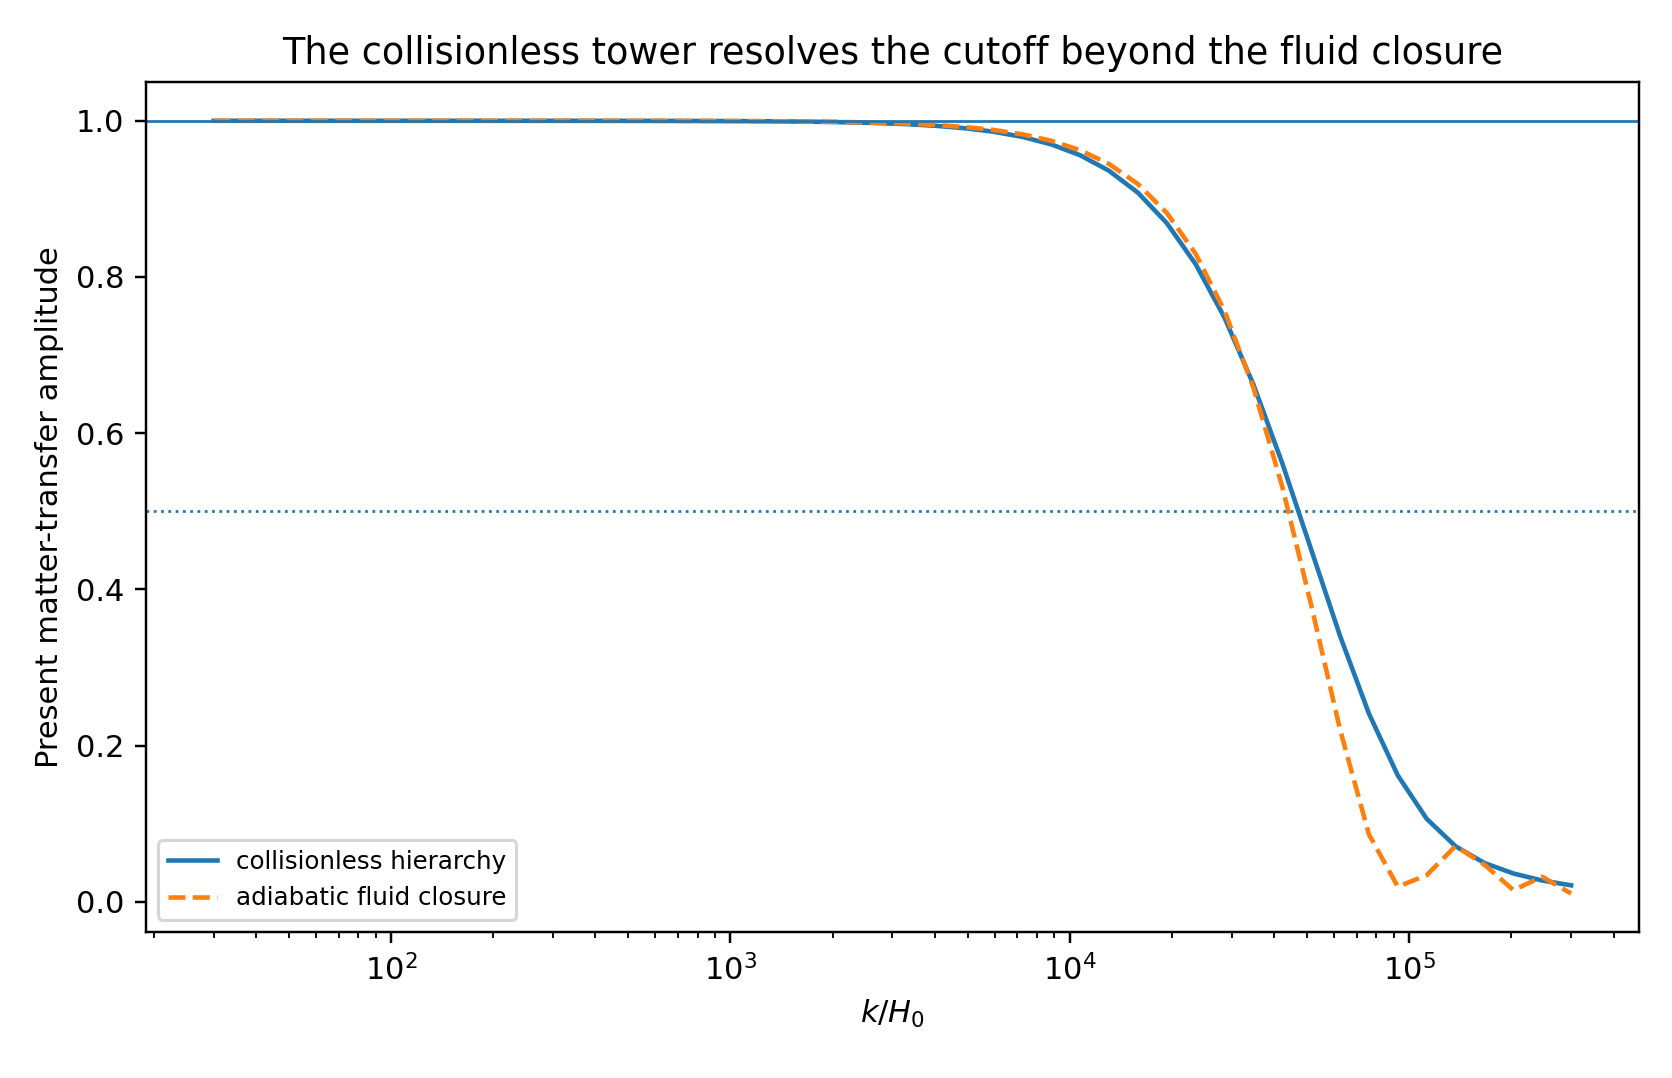
\includegraphics[width=0.88\linewidth]{figures/cb/collisionless_vs_fluid_transfer.png}
\caption{The collisionless hierarchy and the earlier adiabatic-fluid closure agree at large scale but differ materially after free streaming populates higher angular moments.}
\label{fig:cb-collisionless-fluid}
\end{figure}

Selected present values are
\begin{center}
\begin{tabular}{rrrr}
\toprule
$k/H_0$ & $T_m$ & $P_m/P_m^{\rm cold}$ & $T_m^{\rm fluid}$\\
\midrule
$3.15\times10^2$ & 0.999960 & 0.999921 & 0.999967\\
$2.72\times10^3$ & 0.997044 & 0.994096 & 0.997542\\
$2.86\times10^4$ & 0.747869 & 0.559307 & 0.756672\\
$5.14\times10^4$ & 0.451041 & 0.203438 & 0.380038\\
$9.26\times10^4$ & 0.161800 & 0.026179 & 0.019458\\
$3.00\times10^5$ & 0.021197 & 0.000449 & 0.010676\\
\bottomrule
\end{tabular}
\end{center}
The hierarchy is not equivalent to replacing the distribution by a single sound speed.  The difference changes sign across the cutoff because the collisionless response contains phase mixing rather than one coherent acoustic oscillation.

\section{Redshift-space growth and anisotropic stress}

On the common logarithmic scale-factor grid, define
\begin{equation}
 f_m(k,a)=\frac{d\log\delta_m(k,a)}{d\log a}.
 \label{eq:cb-growth-rate}
\end{equation}
For equal primordial normalization, the scale-dependent redshift-space amplitude ratio is
\begin{equation}
 \mathcal R_{f\sigma_8}(k,a)
 =\frac{f_m\delta_m}{f_m^{\rm cold}\delta_m^{\rm cold}}.
 \label{eq:cb-fsigma-ratio}
\end{equation}
At $z=0$, the benchmark gives
\begin{equation}
 \mathcal R_{f\sigma_8}=0.9970
 \quad\text{at}\quad k/H_0\simeq2.72\times10^3,
 \label{eq:cb-fsigma-large}
\end{equation}
\begin{equation}
 \mathcal R_{f\sigma_8}=0.7471
 \quad\text{at}\quad k/H_0\simeq2.86\times10^4,
 \label{eq:cb-fsigma-mid}
\end{equation}
\begin{equation}
 \mathcal R_{f\sigma_8}=0.1603
 \quad\text{at}\quad k/H_0\simeq9.26\times10^4.
 \label{eq:cb-fsigma-small}
\end{equation}
The computed late-time anisotropic stress remains finite and is below $1.5\times10^{-12}$ on the selected observable table.  It is dynamically retained even though it is numerically small for this very cold benchmark.

\begin{figure}[htbp]
\centering
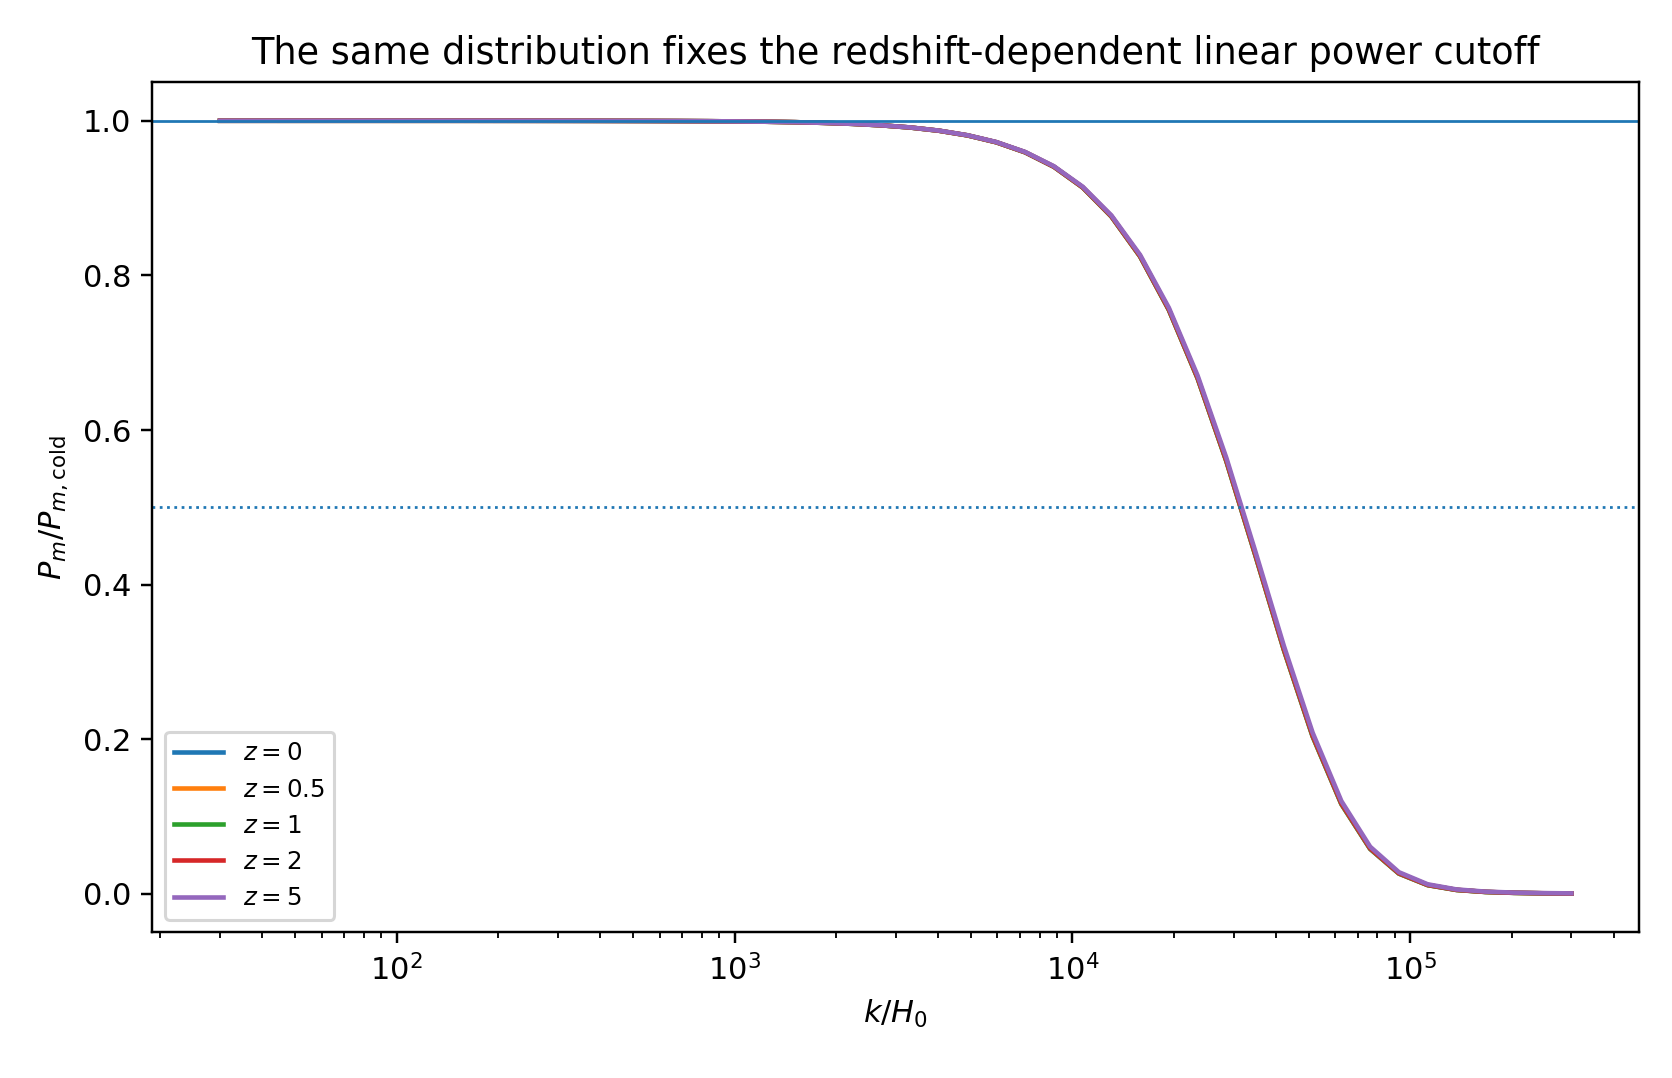
\includegraphics[width=0.88\linewidth]{figures/cb/matter_power_ratio_history.png}
\caption{The power cutoff develops continuously after the declared initial epoch.  The large scales remain locked to the cold reference while the high-$k$ modes lose coherent growth.}
\label{fig:cb-power-history}
\end{figure}

\section{Weak-lensing and CMB-lensing templates}

For a flat source plane at comoving distance $\chi_s$, define the controlled linear lensing ratio
\begin{equation}
 \mathcal R_\ell^\kappa
 =\frac{
 \int_0^{\chi_s}d\chi\,
 W(\chi,\chi_s)^2\chi^{-2}
 P_{\rm cold}(k,z)T_W(k,z)^2
 }{
 \int_0^{\chi_s}d\chi\,
 W(\chi,\chi_s)^2\chi^{-2}
 P_{\rm cold}(k,z)
 },
 \label{eq:cb-lensing-ratio}
\end{equation}
where
\begin{equation}
 k=\frac{\ell+1/2}{\chi}.
 \label{eq:cb-limber-map}
\end{equation}
The reference weight uses the same cold growth and the declared positive equality filter
\begin{equation}
 T_{\rm eq}(k)=\frac{1}{1+(k/k_{\rm eq})^2},
 \qquad
 \frac{k_{\rm eq}}{H_0}=\Omega_{m0}\sqrt{\frac{2}{\Omega_{r0}}}.
 \label{eq:cb-equality-filter}
\end{equation}
This is a normalized linear diagnostic.  It is not a nonlinear shear likelihood and does not include survey masks, intrinsic alignments, nonlinear baryonic feedback, or post-Born corrections.

For a galaxy source at $z_s=0.5$,
\begin{equation}
 \mathcal R_{1000}^{\kappa}=0.981331,
 \qquad
 \mathcal R_{3000}^{\kappa}=0.863481,
 \qquad
 \mathcal R_{5000}^{\kappa}=0.702128.
 \label{eq:cb-lensing-z05}
\end{equation}
For $z_s=1$,
\begin{equation}
 \mathcal R_{1000}^{\kappa}=0.993772,
 \qquad
 \mathcal R_{3000}^{\kappa}=0.949092,
 \qquad
 \mathcal R_{5000}^{\kappa}=0.874908.
 \label{eq:cb-lensing-z1}
\end{equation}
For a CMB source plane at the declared initial redshift $z_s=999$,
\begin{equation}
 \mathcal R_{1000}^{\kappa}=0.999615,
 \qquad
 \mathcal R_{2000}^{\kappa}=0.998474,
 \qquad
 \mathcal R_{3000}^{\kappa}=0.996591.
 \label{eq:cb-cmb-lensing}
\end{equation}

\begin{figure}[htbp]
\centering
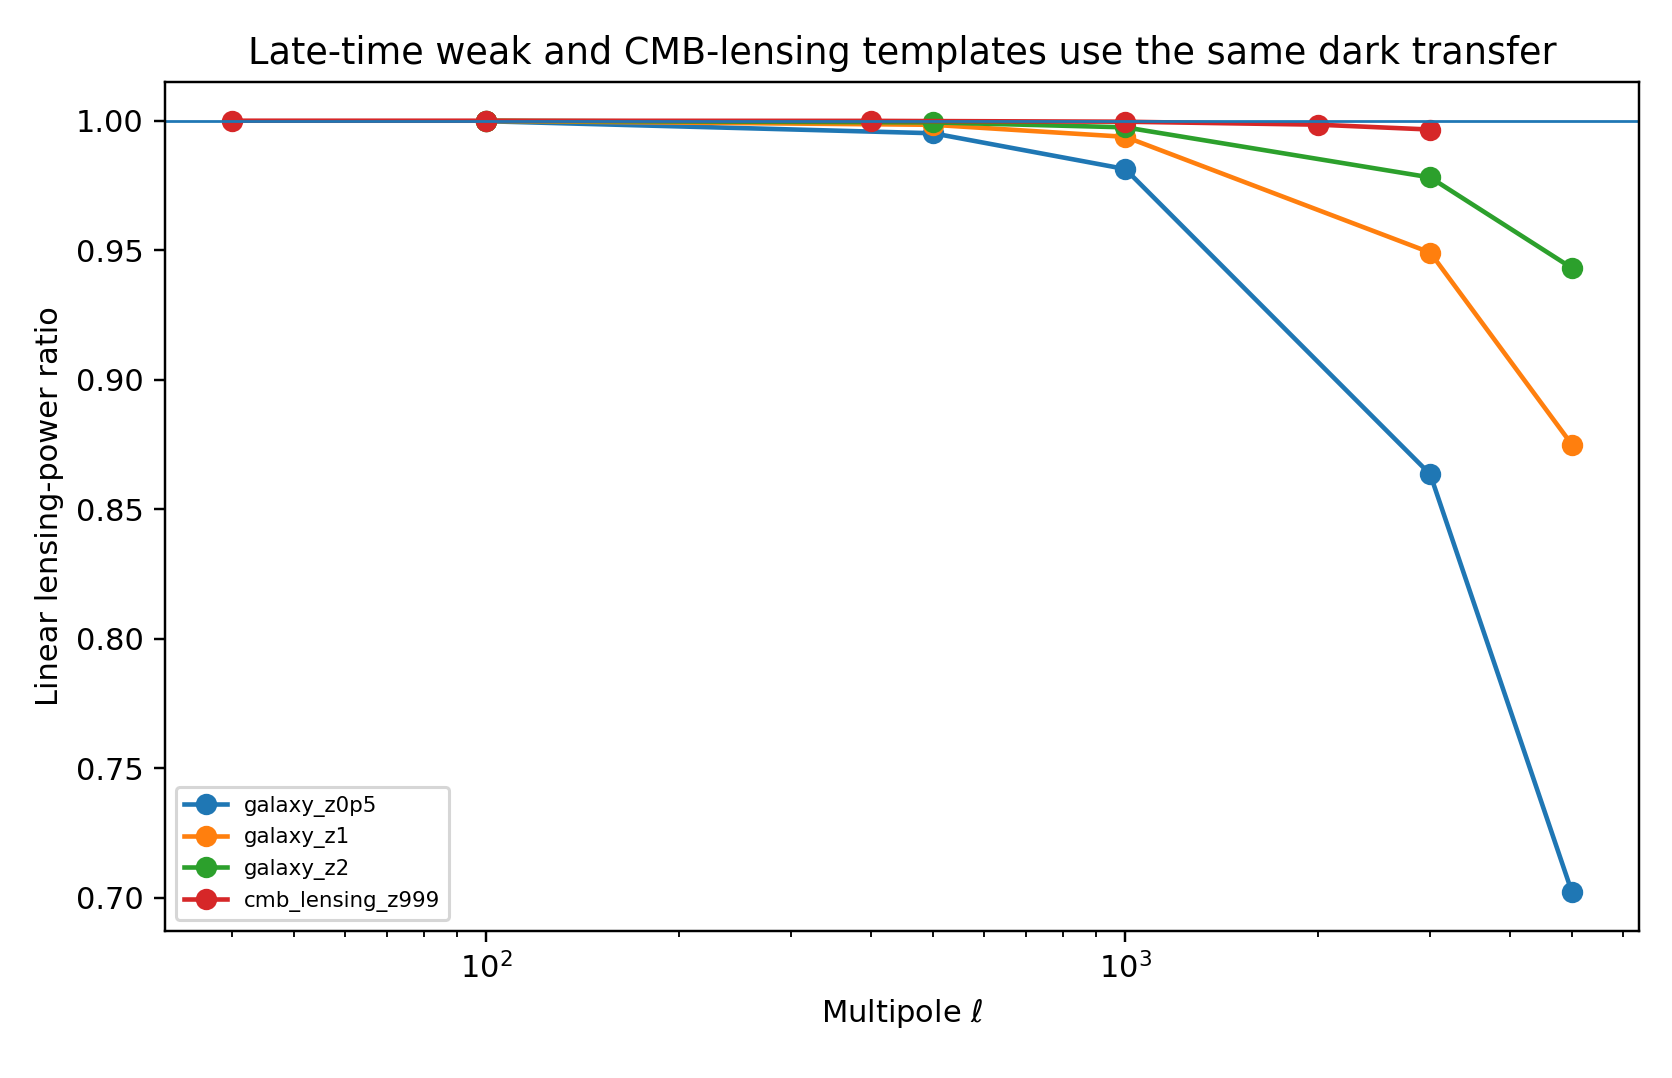
\includegraphics[width=0.88\linewidth]{figures/cb/lensing_power_ratios.png}
\caption{The late-time linear lensing response follows from the same collisionless Weyl transfer function without changing the dark parameters between clustering and lensing.}
\label{fig:cb-lensing-ratios}
\end{figure}

\section{Primary-CMB scale separation}

The comoving distance of the controlled background to $a=10^{-3}$ maps $\ell=3000$ to
\begin{equation}
 \left.\frac{k}{H_0}\right|_{\ell=3000}
 =957.699.
 \label{eq:cb-primary-k}
\end{equation}
This is only
\begin{equation}
 \boxed{
 \frac{k_{\ell=3000}}{k_{1/2}^{(P)}}=0.0304481}
 \label{eq:cb-primary-half-ratio}
\end{equation}
of the late-time power half-mode.  Thus the declared cutoff is parametrically separated from the primary acoustic scale.  This does not replace a primary TT, TE, or EE calculation.  It shows only a scale separation inside the declared late-time model.  Pre-$a_i$ free streaming, photon and neutrino metric driving, and recombination physics must be evolved before any statement about primary anisotropies is justified.

\section{Verification ledger}

The deterministic implementation records
\begin{equation}
 \boxed{20\ \mathrm{PASS},\qquad0\ \mathrm{FAIL}.}
 \label{eq:cb-check-count}
\end{equation}
The principal numerical controls are
\begin{center}
\begin{tabular}{lrr}
\toprule
control & coarse difference & fine difference\\
\midrule
momentum quadrature & $1.41\times10^{-4}$ & $3.05\times10^{-5}$\\
multipole truncation & $3.62\times10^{-5}$ & $3.62\times10^{-5}$\\
time-step refinement & $5.41\times10^{-8}$ & $1.89\times10^{-8}$\\
cold-production limit & -- & $4.01\times10^{-4}$\\
\bottomrule
\end{tabular}
\end{center}
The time-step sequence has an effective fitted order $1.52$ at the reported precision because the remaining error is already dominated by the moving angular closure and phase-space truncation.  The fine transfer difference itself is below $2\times10^{-8}$.

\section{Closure ledger}

\begin{center}
\begin{tabular}{>{\raggedright\arraybackslash}p{0.48\linewidth}>{\raggedright\arraybackslash}p{0.21\linewidth}>{\raggedright\arraybackslash}p{0.23\linewidth}}
\toprule
statement & status & boundary\\
\midrule
massive collisionless hierarchy for every retained level and momentum node & derived and implemented & linear perturbations\\
phase-space stress tensor including anisotropic stress & closed & declared quadrature\\
self-consistent baryon--tower Poisson source & closed controlled & quasi-static post-recombination regime\\
large-scale cold limit & numerically closed & declared hierarchy grid\\
post-recombination incremental transfer cutoff & numerically closed & prescribed data at $a_i$\\
scale-dependent $f\sigma_8$ template & closed controlled & linear theory\\
galaxy weak-lensing ratio & closed controlled & linear Limber template\\
CMB-lensing ratio & closed controlled & linear late-time lensing only\\
primary TT, TE, EE spectra & open & photon collisions and polarization\\
massless-neutrino hierarchy and recombination coupling & open & full Einstein--Boltzmann system\\
nonlinear matter power and halo formation & open & nonlinear solver or calibrated emulator\\
observational likelihood and parameter inference & open & external data and nuisance model\\
\bottomrule
\end{tabular}
\end{center}

\section{Synthesis and unresolved requirements}

The scale-covariant refinement distribution now determines, without replacing it by one sound speed,
\begin{equation}
 \boxed{
 \bar f_h(q)
 \Longrightarrow
 \{F_{h\ell}(q,k,a)\}
 \Longrightarrow
 \{T_m,T_W,f\sigma_8,\mathcal R_\ell^\kappa\}.}
 \label{eq:cb-result-chain}
\end{equation}
The same mass spectrum and production scale control dark clustering, redshift-space growth, galaxy lensing, and CMB lensing.

The unresolved kinetic and observational requirements are:
\begin{equation}
 \boxed{
 \begin{gathered}
 \text{add photons, polarization, baryons, and massless neutrinos},\\
 \text{couple the hierarchy through recombination and reionization},\\
 \text{compute TT, TE, EE, lensing, and }P_m(k)\text{ together},\\
 \text{then perform one joint likelihood without retuning the dark sector}.
 \end{gathered}}
 \label{eq:cb-open-requirements}
\end{equation}
